
\documentclass[12pt,letterpaper,noanswers]{exam}
\usepackage[usenames,dvipsnames,svgnames,table]{xcolor}
\usepackage[margin=0.9in]{geometry}
\renewcommand{\familydefault}{\sfdefault}
\usepackage{multicol}
\pagestyle{head}
\header{AM 111 Class 15}{}{Approximating integrals, p.\thepage}
\runningheadrule
\headrule
\usepackage{siunitx}
\usepackage{graphicx} % more modern
\usepackage{amsmath} 
\usepackage{amssymb} 
\usepackage{hyperref}
\usepackage{tcolorbox}
\usepackage{listings}
%\usepackage[numbered,autolinebreaks,useliterate]{mcode}

\usepackage{enumitem}
\def\mbf{\mathbf}
\newcommand{\vc}[1]{\boldsymbol{#1}}
\def\dsst{\displaystyle}
\DeclareMathOperator*{\argmin}{arg\,min} % thin space, limits underneath in displays


\begin{document}
 \pdfpageheight 11in 
  \pdfpagewidth 8.5in

\noindent 

\section*{Preliminaries}

\begin{itemize}
\itemsep0pt
\item There is a problem set due Friday.
\item There is a skill check in the next class.
\end{itemize}


\noindent\textbf{Big picture}

Today: Approximating $\int_{a}^{b}f(x)dx$.

\vspace{0.2cm}
\hrule
\vspace{0.2cm}

\noindent \textbf{Skill check practice}

 The error from using the trapezoid rule to approximate $\int_a^b f(x)dx$ with a single panel is given by $-\frac{1}{12}h^3f''(c_1)$, where $h$ is the panel size.  What is the error for the composite rule?



\vspace{0.2cm}
\hrule
\vspace{0.2cm}

\noindent \textbf{Skill check solution}

Explanation:

For $m$ panels evenly splitting $[a,b]$, this comes from $\sum\limits_{k=1}^m -\frac{1}{12}h^3f''(c_k) = -\frac{1}{12}mh^3f''(c) = -\frac{1}{12}(b-a)h^2f''(c)$ (from the generalized intermediate value theorem and assuming $mh = (b-a)$).


Answer:

 $-\frac{1}{12}(b-a)h^2f''(c)$.  


General case:

In general for error $\alpha h^nf^{(k)}(c_1)$ on a single panel of size $h$, the error will be $\alpha (b-a)h^{n-1}f^{(k)}(c)$ for the composite rule.


\vspace{0.2cm}
\hrule
\vspace{0.2cm}






\subsection*{Gaussian quadrature (following Sauer \S5.5)}


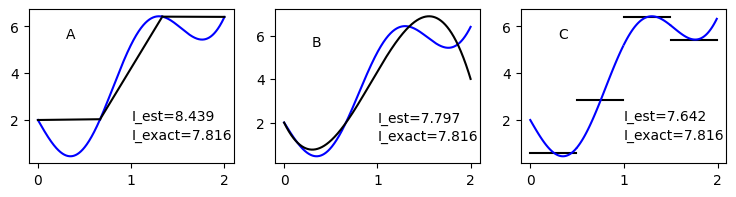
\includegraphics[width=\linewidth]{img/C17estimates.png}
\begin{enumerate}[resume=classQ]
\item In the figure above, the integral $\displaystyle I_{\text{exact}} = \int_0^2 \left(e^x - 2\cos(4x) + 1\right) dx\approx 7.816$.  Note that this function is transcendental and not a polynomial.

The value of the integral is estimated via different quadrature rules.  Each estimate is using exactly four function evaluations.
\begin{parts}
\item For each method, $\displaystyle I_\text{estimate} = \int_0^2 p(x)dx$ for some function $p(x)$.  The function $p(x)$ is shown in black for each method.  How many panels appear to be used for each estimate?

\begin{tabular}{c | p{1.5cm} p{1.5cm} p{1.5cm}}
figure &A &B&C \\
\hline
& & & \\
\# panels &\\
&\\
\end{tabular}
\item Assuming there are $k$ function evaluations associated with each panel (some of these function evaluations may be used in multiple panels), identify $k$. 

\begin{tabular}{c | p{1.5cm} p{1.5cm} p{1.5cm}}
figure &A &B&C \\
\hline
& & & \\
$k$ &\\
&\\
\end{tabular}
\item The three quadrature methods used are: composite midpoint, composite trapezoid, Gaussian quadrature on $4$ points.  Match the method to the plot.
\vspace{1in}
\item Which method is has the minimum error for this problem?
\vspace{1cm}
\item The theoretical error bounds are $-\frac{1}{12}(b-a)h^2f''(c)$ (composite trapezoid), $\frac{1}{24}(b-a)h^2f''(c)$ (composite midpoint)

\end{parts}
\end{enumerate}


\begin{tcolorbox}

\begin{itemize}
\itemsep0pt
    \item A Newton-Cotes method using a quadrature of degree $n$ has degree of precision $n$ for $n$ odd and $n+1$ for $n$ even.
    \item The Trapezoid rule ($n = 1$, two points) has degree of precision $1$.
    \item Simpson's rule ($n=2$, three points) has degree of precision $3$.
    \item These methods use $n+1$ function evaluations.
\end{itemize}
\textbf{Gaussian quadrature} has degree of precision $2n-1$ when $n$ points are used.
\end{tcolorbox}
\begin{enumerate}[resume=classQ]
    \item Consider $I = \int_a^b f(x)dx$.  Let $g(x) = f(x+h+a)$, $h = (b-a)/2$.  $I = \int_{-h}^h g(x) dx$.
    
        $\int_{-h}^h g(x) dx \approx c_1 g(x_1) + c_2 g(x_2)$.  We would like to $c_1, c_2, x_1, x_2$ to maximize the degree of precision of this method.  
        
        With four unknowns that we can set, the method should be exactly correct for $g(x) = 1, x, x^2, x^3$ (degree of precision of $3$).
    \begin{parts}
\item Assuming a degree of precision of $3$, find four equations that are satisfied by $c_1, c_2, x_1, x_2$.
\vspace{1.5in}
\item This is a system of nonlinear equations.  Make an effort to find a solution to the system (you might use that $c_1x_1 = -c_2x_2$).  \emph{It is typically difficult to find a solution to a nonlinear system}.

\vspace{3in}

\item If you were to use $n$ points instead of $2$ points, how many unknowns would you have?  What degree of precision is possible (assuming the system you generate has a solution)?
\end{parts}
\end{enumerate}


\begin{tcolorbox}
\begin{itemize}
\itemsep0pt
    \item For an $n$ point Gaussian quadrature method, choosing the right $x_k$ is a little complicated.
    \item Once the $x_k$ are chosen, we can use Lagrange interpolation to find the quadrature weights.  %set up Lagrange basis functions $\displaystyle L_k(x) = \prod\limits_{j=1, j\neq k}^n \dfrac{x-x_j}{x_k-x_j}$
\end{itemize}

\end{tcolorbox}

\begin{enumerate}[resume=classQ]
\item You are using an $n$ point quadrature method.  Assume you have been told to use points $x_1, x_2, ..., x_n$ (where the $x_k$ values are given to you) to create an interpolating polynomial.

Let $L_k(x)$ be the basis functions for Lagrange interpolation, so $g(x) = \sum\limits_{k=1}^n f(x_k) L_k(x)$

Write an expression to find $c_k$ where $\displaystyle\int_{-h}^h g(x) dx \approx \sum\limits_{k=1}^n c_k f(x_k)$.

\emph{Note: your expression will involve an integral}

\vspace{1in}



%$\int_{-h}^h y_k L_k(x) dx = \sum\limits_{k=1}^n y_k\int_{-h}^h L_k(x) dx$

\end{enumerate}
\begin{tcolorbox}
(from Greenbaum and Chartier \S 10.3.1)

Let $\{p_0(x),p_1(x),...,p_k(x),...,p_n(x)\}$ be a set of orthogonal polynomials on the interval $[-h,h]$ with $p_k$ of degree $k$.
\begin{itemize}
\itemsep0pt
    \item Set the $x_i$ to be the roots of $p_n(x)$. Then for $j\leq 2n-1$, $\displaystyle \int_{-h}^h x^j dx = \sum\limits_{i=1}^n c_i x_i^j$, i.e. the quadrature has a degree of precision of $2n-1$.
    \item The quadrature created using Lagrange interpolation at these roots $x_i$ is the \textbf{Gaussian quadrature}.
\end{itemize}

Proof: Via polynomial long division, $x^j = q_{n-1}p_n + r_{n-1}$ where $q_{n-1}$ and $r_{n-1}$ have degree at most $n-1$.  We have $p_n(x_i) = 0$ so $x_i^j = q_{n-1}(x_i)p_n(x_i) + r_{n-1}(x_i) = r_{n-1}(x_i)$.  Because $q_{n-1}$ is lower degree than $p_n$ it must be orthogonal.  That means we also have $\int_{-h}^h x^j dx = \int_{-h}^h q_{n-1}(x)p_n(x)dx + \int_{-h}^h r_{n-1}(x)dx = \int_{-h}^h r_{n-1}(x) dx$.  By the construction of $c_i$ via Lagrange interpolation, we know the interpolation rule is exact for polynomials of degree $n-1$ or less, so $\int_{-h}^h f(x) dx = \sum\limits_{i=1}^n c_i x_i^j$.

This proof is one of the questions below.

\end{tcolorbox}
\begin{enumerate}[resume=classQ]
\item %Let $P(x)$ be a polynomial of degree at most $2n-1$.

(What are orthogonal polynomials?)

Let $\{p_0(x),p_1(x),...,p_k(x),...,p_n(x)\}$ be a set of orthogonal polynomials on the interval $[-h,h]$ with $p_k$ of degree $k$.
\begin{parts}
\item Two polynomials, $f(x)$ and $g(x)$, are orthogonal on an interval $[-h,h]$ if 

$\displaystyle\int_{-h}^h f(x)g(x)dx = 0$.  Show that $p_0(x) = 1$ and $p_1(x) = x$ are orthogonal on $[-1,1]$.
\vspace{1in}
\item Let $p_2(x) = x^2 + c$.  Find $c$ so that $p_2(x)$ is orthogonal to $p_1(x)$ and to $p_0(x)$.
\vspace{1in}

\end{parts}
\end{enumerate}
\begin{tcolorbox}
Theorems (see Sauer \S 5.4)

\begin{itemize}
\itemsep0pt
    \item Let $\{p_0(x),p_1(x),...,p_k(x),...,p_n(x)\}$ be a set of orthogonal polynomials on the interval $[-h,h]$ with $p_k$ of degree $k$.  Such a set of polynomials is a \textbf{basis} for the vector space of degree at most $n$ polynomials on $[-h,h]$.
    \item If $\{p_0(x),p_1(x),...,p_k(x),...,p_n(x)\}$ is an orthogonal set of polynomials on $[-h,h]$ and if degree $p_k = k$ then $p_k$ has $k$ distinct roots in the interval $(-h,h)$.
    \item The set of \textbf{Legendre polynomials} $\displaystyle p_k(x) = \frac{1}{2^kk!}\frac{d^k}{dx^k}\left[(x^2-1)^k\right]$ forms such an orthogonal basis (on $[-1,1]$).
\end{itemize}
\end{tcolorbox}
\begin{enumerate}[resume=classQ]
    \item Set the $n$ values of $x_i$ to be the roots of $p_n(x)$.  Using polynomial long division, $x^j = S(x)p_n(x) + R(x)$ where $j \leq 2n-1$, $S(x)$ is degree at most $n-1$ and $R(x)$ is the remainder so also degree at most $n-1$.
    \begin{parts}
    \item Write $S(x) = \sum\limits_{i=1}^{n-1} a_i p_i(x)$.  How do you know it is possible to write $S(x)$ in this way?
    \vspace{1cm}
    \item Find $\int_{-1}^1 S(x)p_n(x)dx$.  \emph{By orthogonality, you know $\int_{-1}^1 p_i(x)p_n(x)dx$.}
    \vspace{1in}
 
 You should find that $\int_{-1}^1 x^j dx = \int_{-1}^1 R(x)dx$.  $R(x)$ is of degree $n-1$ or less, so an interpolating polynomial on $n$ points will exactly match it.  
 
 \item Argue that $\int_{-1}^1 x^j dx$ is equal to the quadrature rule applied to $R(x)$, so $\sum\limits_{i=1}^n c_i R(x_i)$.
 \vspace{1cm}
 
 \item Now consider the quadrature rule applied to $x^j = S(x)p_n(x) + R(x)$.  For $x_i$ the roots of $p_n(x)$ simplify $S(x_i)p_n(x_i) + R(x_i)$.
 \vspace{1cm}
    \end{parts}
\end{enumerate}
\begin{tcolorbox}
For any polynomial $P(x)$ of degree $\leq 2n-1$, $P(x) = S(x)p_n(x) + R(x)$.  $\displaystyle\int_{-1}^1 P(x)dx = \int_{-1}^1 R(x)dx = \sum\limits_{i=1}^n c_i R(x_i)$ where the $x_i$ are the $n$ roots of $p_n(x)$.

The Gaussian quadrature has a degree of precision of $2n-1$.
\end{tcolorbox}


% \subsection*{Romberg Integration}

% \been

% \item[4.] Romberg integration uses the composite trapezoid rule with successively
% smaller stepsizes $h$.

% \been
% \item {\bf Romberg Integration (First Column)}

% Define stepsizes $h_j$ such that each successive stepsize is half the
% previous stepsize:
% \begin{align*}
% h_1 &= b-a \\
% h_2 &= (b-a)/2 \\ 
% h_3 &= (b-a)/4 \\
% & \vdots \\
% h_j&=\frac{1}{2^{j-1}}(b-a).
% \end{align*}

% The first column of Romberg integration, $R_{j1}$, is the composite
% trapezoid rule applied to the function on $[a,b]$ with stepsize $h_j$.  Write down the formula for the first few elements of the first column:

% \vfill

% \begin{align*}
% R_{11} &= \blank{3in} \\
% & \\
% R_{21} &= \blank{3in} \\
% & \\
% R_{31} &= \blank{3in}
% \end{align*}

% \pagebreak

% The second column applies Richardson extrapolation to the 1st column
% $R_{j1}$.  Write down the results for the second column.  What is $R_{22}$?

% \vfill

% \begin{align*}
% R_{22} &= \frac{2^2 R_{21} - R_{11}}{3} = \blank{3in} \\
% & \\
% R_{32} &= \frac{2^2 R_{31} - R_{21}}{3} = \blank{3in}
% \end{align*}

% \item Calculate $R_{11}$, $R_{21}$, and $R_{22}$ for $\dsst{\int_0^4 x^2 \, dx}$.

% \vfill

% \pagebreak

% \item The third column applies Richardson extrapolation to the second column.
% Because the second column is composite Simpson's rule, it is 4th order in $h$:
% \begin{align*}
% R_{33} &= \frac{4^2 R_{32} - R_{22}}{4^2-1} \\
% R_{43} &= \frac{4^2 R_{42} - R_{32}}{4^2-1} \\
% & \vdots \\
% R_{j3} &= \frac{4^2 R_{j2} - R_{j-1,2}}{4^2-1}
% \end{align*}

% \item This pattern perpetuates
% $$
% R_{jk} = \frac{4^{k-1} R_{j,k-1} - R_{j-1,k-1}}{4^{k-1}-1} 
% $$

% \enen

% \item[5.] Computer Examples
% \been

% \item Estimate $\dsst{\int_{-1}^1 2\sqrt{1-x^2} \, dx}$.

% \vspace{1cm}

% \item Estimate $\dsst{\int_{-1}^1 1 + \sin{e^{3x}} \, dx}$.

% \vspace{1cm}

% \enen

% \enen



\subsection*{Adaptive quadrature}

\begin{lstlisting}
% From Sauer: program 5.2 Adaptive Quadrature
% Computes approximation to definite integral
% Inputs: Matlab function f, interval [a0,b0], 
%   error tolerance tol0
% Output: approximate definite integral
function sum = adapquad(f,a0,b0,tol0)
sum=0; 
n=1; 
a(1)=a0; 
b(1)=b0; 
tol(1)=tol0; 
app(1)=trap(f,a,b);
% n is current position at end of the list
while n>0           
  c = (a(n)+b(n))/2;
  oldapp = app(n);
  app(n) = trap(f,a(n),c);
  app(n+1) = trap(f,c,b(n));
  if abs(oldapp-(app(n)+app(n+1))) < 3*tol(n)
    % success
	sum = sum + app(n) + app(n+1);
	% done with interval
	n = n-1;                         
  else
    % divide into two intervals
    % set up new intervals
	b(n+1)=b(n); 
	b(n)=c;
	a(n+1)=c;
	tol(n)=tol(n)/2; tol(n+1)=tol(n);
	% go to end of list, repeat
	n=n+1;                         
  end
end

function s=trap(f,a,b)
s = (f(a)+f(b))*(b-a)/2;

\end{lstlisting}

\begin{enumerate}[resume=classQ]
\item Let $I = \displaystyle\int_0^1 x^2 dx$.  For your reference, $I = 1/3$.
\begin{parts}
\item Call \texttt{adapquad(f,0,1,0.01)}.  In the first column, follow each of the variables on the first pass through the loop.  As a variable updates, cross out the old value and write the new one.

Trace the program for the first time through the loop.

Then trace again for the second pass through the loop.

\begin{tabular}{l|p{5cm} | p{5cm}| c}
variable & time 1 & time 2 & ...\\
\hline
& && \\
sum & && \\
& &&\\
n & && \\ & &&\\
a & && \\ & &&\\
b & && \\ & &&\\
tol & & &\\ & &&\\
app & && \\ & &&\\
c & && \\ & &&\\
oldapp & && \\%& &&\\

\end{tabular}

\item What does this code do?  Why is the method called \emph{adaptive}?
\vspace{1in}

\end{parts}
\end{enumerate}



\end{document}